\chapter{Analisis}
\label{chap:analisis}

Bab ini membahas analisis yang menjadi dasar perancangan dan pengembangan aplikasi desktop pemeriksa tautan rusak pada situs web. Analisis mencakup permasalahan utama yang melatarbelakangi penelitian, tinjauan terhadap sistem serupa, serta perumusan kebutuhan sistem baik fungsional maupun non-fungsional. Selain itu, dibahas pula analisis terhadap teknologi yang digunakan untuk mendukung implementasi aplikasi.

\section{Analisis Masalah}
\label{sec:03-analisis-masalah}
% \subsection{Tautan Rusak}
\label{subsec:0301-tautan-rusak}

Analisis mengenai tautan rusak pada penelitian ini didasarkan pada teori URI yang dijelaskan pada Subbab~\ref{sec:02-uri} serta teori HTTP pada Subbab~\ref{sec:02-http}. Tujuan utamanya adalah memahami faktor-faktor yang membuat tautan gagal diakses. Dengan melihat struktur URL, aturan sintaks, mekanisme resolusi, hingga kode status HTTP, kita dapat memahami dengan lebih jelas bagaimana tautan dinyatakan rusak dan apa saja indikator yang bisa digunakan untuk mengenalinya.

\subsubsection*{Struktur URL}
Pada Subbab~\ref{subsec:0202-struktur-url} dijelaskan bahwa URL memiliki sejumlah komponen, mulai dari \textit{scheme}, \textit{host}, \textit{port}, \textit{path}, \textit{query}, hingga \textit{fragment}. Dari sisi analisis, tidak semua bagian berpengaruh langsung pada keabsahan tautan. Komponen yang paling menentukan adalah \textit{scheme}, \textit{host}, \textit{port}, \textit{path}, dan \textit{query}, sedangkan \textit{fragment} hanya diproses di sisi klien.

Beberapa contoh permasalahan yang bisa muncul:
\begin{itemize}
  \item \textbf{Scheme} yang salah membuat agen pengguna tidak bisa membangun koneksi.
  \item \textbf{Host} yang keliru, misalnya domain salah ketik atau tidak terdaftar, menyebabkan tautan tidak ditemukan.
  \item \textbf{Port} yang tidak sesuai membuat layanan yang dituju tidak dapat diakses.
  \item \textbf{Path} yang tidak valid biasanya mengembalikan respons \texttt{404 Not Found}.
  \item \textbf{Query} yang salah dapat membuat server gagal menampilkan hasil yang diinginkan.
\end{itemize}

Dari sini terlihat bahwa kesalahan pada salah satu komponen utama sudah cukup untuk membuat tautan tidak berfungsi.

\subsubsection*{Validitas Sintaks dan Encoding}
Aturan penggunaan karakter dalam URI dan mekanisme \textit{percent-encoding} dibahas pada Subbab~\ref{subsec:0202-karakter-percent-encoding}. Dalam praktiknya, banyak tautan yang rusak bukan karena salah struktur, tetapi karena melanggar aturan sintaks atau \textit{encoding}. Contoh yang sering terjadi adalah penggunaan karakter \textit{reserved} di luar konteks, adanya spasi atau karakter non-ASCII yang tidak dikodekan, atau penulisan \textit{percent-encoding} dengan format yang salah.

Masalah lain muncul dari normalisasi, sebagaimana dijelaskan pada Subbab~\ref{subsec:0202-normalisasi-url}. Misalnya \textit{host} ditulis dengan huruf besar, port default tetap dicantumkan, atau path masih berisi segmen \texttt{.} dan \texttt{..}. Situasi semacam ini membuat URL ambigu. Artinya, meskipun sebuah URL terlihat benar, kesalahan kecil dalam sintaks atau encoding bisa membuatnya dianggap rusak.

\subsubsection*{URL Relatif}
Pada Subbab~\ref{subsec:0202-struktur-url} dijelaskan bahwa URL relatif harus digabungkan dengan \textit{base URI} untuk membentuk URL absolut. Masalah muncul ketika \textit{base URI} tidak jelas atau proses resolusinya tidak berjalan dengan benar. Hasilnya, URL absolut yang terbentuk tidak menunjuk ke sumber daya yang diinginkan.

Hal serupa bisa terjadi bila \textit{dot-segments} tidak dihapus. Akibatnya, jalur yang terbentuk tidak sesuai. Dalam kondisi ini, tautan yang seharusnya valid sebagai URL relatif menjadi tidak dapat digunakan setelah diubah menjadi absolut.

\subsubsection*{Komunikasi HTTP}
HTTP sebagai protokol komunikasi dibahas pada Subbab~\ref{sec:02-http}. Walaupun sebuah URL valid secara struktur, tautan tetap bisa gagal diakses bila komunikasi HTTP tidak berhasil. Permasalahan ini biasanya muncul pada tahap koneksi antara klien dan server.

Beberapa kasus yang sering ditemui adalah:
\begin{itemize}
  \item \textbf{Host tidak ditemukan}, misalnya ketika domain gagal dipetakan oleh DNS.
  \item \textbf{Koneksi ditolak}, ketika server tidak menyediakan layanan pada port yang diminta.
  \item \textbf{Timeout}, ketika server tidak memberikan respons dalam batas waktu yang ditentukan.
\end{itemize}

Dengan kata lain, validitas URL belum cukup. Tautan juga perlu diuji pada tahap komunikasi, karena kegagalan di sini tetap membuatnya rusak.

\subsubsection*{Kode Status HTTP}
Pada Subbab~\ref{subsec:0201-kode-status-http} dijelaskan bahwa setiap respons HTTP memiliki kode status sebagai penanda hasil permintaan. Dalam analisis tautan rusak, kode inilah yang biasanya menjadi acuan utama.

Beberapa kategori kode status yang sering digunakan adalah:
\begin{itemize}
  \item \textbf{4xx Client Error}. Kategori ini menandakan kesalahan di sisi klien. Contoh yang paling sering ditemui adalah \texttt{404 Not Found}. Ada juga \texttt{410 Gone} yang berarti sumber daya sudah dihapus secara permanen, serta \texttt{403 Forbidden} ketika akses ditolak.
  \item \textbf{5xx Server Error}. Kategori ini menunjukkan kegagalan di sisi server. Misalnya \texttt{500 Internal Server Error} yang menandakan adanya masalah umum pada server, atau \texttt{503 Service Unavailable} ketika layanan tidak tersedia untuk sementara.
  \item \textbf{Redirect loop}. Kondisi ini muncul ketika server berulang kali mengarahkan ke lokasi lain dengan kode 3xx tanpa pernah benar-benar sampai ke sumber daya tujuan.
\end{itemize}

Dari sini dapat dipahami bahwa kode status HTTP bukan hanya informasi teknis, tetapi juga indikator praktis untuk menentukan apakah sebuah tautan masih berfungsi atau sudah masuk kategori rusak.

\subsection{\textit{Web Crawling}}
\label{subsec:0301-web-crawlin}

Analisis pada bagian ini merujuk pada teori mengenai \textit{web crawling} yang dibahas pada Subbab~\ref{sec:02-web-crawling} serta teori HTML pada Subbab~\ref{sec:02-html}. Tujuan utamanya adalah mengidentifikasi permasalahan yang muncul dalam proses \textit{crawling} halaman web sebagai dasar pemeriksaan tautan rusak. Permasalahan tersebut mencakup strategi \textit{crawling}, jenis \textit{crawler} yang digunakan, tantangan teknis yang dihadapi, serta keterkaitannya dengan struktur HTML sebagai sumber tautan.

\subsubsection*{Strategi \textit{crawling}}
Pada Subbab~\ref{sec:02-web-crawling} dijelaskan bahwa strategi \textit{crawling} dapat dilakukan dengan \textit{breadth-first crawling} maupun \textit{na\"{i}ve best-first crawling}. Keduanya memiliki karakteristik yang berbeda.  

\begin{itemize}
  \item \textbf{\textit{Breadth-first crawling}} menyapu halaman secara merata dari titik awal. Strategi ini cocok digunakan untuk aplikasi pemeriksa tautan, karena setiap halaman pada host yang sama dianggap memiliki tingkat kepentingan yang setara. Dengan cara ini, cakupan situs dapat diperoleh lebih menyeluruh tanpa harus memikirkan bobot prioritas antar tautan.
  \item \textbf{\textit{Na\"{i}ve best-first crawling}} menggunakan \textit{priority queue} berbasis skor untuk menentukan halaman yang akan diambil lebih dahulu. Strategi ini bermanfaat bila ada kriteria relevansi yang jelas, misalnya hanya ingin menekankan halaman dengan potensi informasi lebih tinggi. Namun, dalam konteks aplikasi pemeriksa tautan rusak, pendekatan ini tidak relevan. Semua halaman pada satu host dianggap sama penting, sehingga tidak ada dasar untuk memberikan skor prioritas.
\end{itemize}

Dengan demikian, strategi yang logis untuk aplikasi ini adalah \textit{breadth-first crawling}.

\subsubsection*{Jenis Crawler}
Subbab~\ref{sec:02-web-crawling} juga membahas jenis-jenis \textit{crawler}, seperti \textit{universal crawler}, \textit{focused crawler}, dan \textit{topical crawler}.  

\begin{itemize}
  \item \textbf{\textit{Universal crawler}} mencoba merayapi seluruh bagian web dalam skala luas. Jenis ini tidak sesuai untuk aplikasi pemeriksa tautan karena lingkupnya terlalu besar dan tidak efisien.
  \item \textbf{\textit{Focused crawler}} membatasi diri pada kriteria tertentu. Pendekatan ini relevan karena aplikasi ini hanya perlu merayapi halaman dengan host yang sama. Dengan cara ini, proses \textit{crawling} lebih terarah dan sumber daya tidak terbuang pada tautan eksternal.
  \item \textbf{\textit{Topical crawler}} memfokuskan \textit{crawling} pada topik tertentu. Jenis ini biasanya digunakan untuk pengumpulan konten tematik. Untuk pemeriksa tautan, pendekatan ini tidak diperlukan karena tujuan utamanya adalah validitas tautan, bukan isi konten.
\end{itemize}

Dengan pertimbangan tersebut, aplikasi pemeriksa tautan lebih sesuai menggunakan pendekatan \textit{focused crawling} dengan batasan pada domain yang sama.

\subsubsection*{Tantangan Teknis}
Subbab~\ref{subsec:0204-tantangan-crawling} menjelaskan sejumlah tantangan yang umum dihadapi dalam \textit{crawling}. Dalam sistem yang dikembangkan, setiap tantangan tersebut ditinjau kembali dan ditetapkan keputusan penerapannya sebagai berikut:

\begin{itemize}
  \item \textbf{\textit{Fetching}}: dalam sistem ini akan diterapkan pengaturan \textit{timeout} agar proses tidak berhenti terlalu lama pada tautan yang tidak merespons. Selain itu, akan ada jeda antar permintaan sebagai bentuk pengendalian agar server tidak terbebani dan tidak memblokir pemeriksaan.
  
  \item \textbf{\textit{Parsing}}: dalam sistem ini akan digunakan Jsoup untuk mengurai HTML. Parser ini dipilih karena mampu menangani dokumen dengan struktur yang tidak sempurna, sehingga tautan tetap dapat diekstrak. Namun, tautan yang dihasilkan secara dinamis melalui JavaScript tidak akan diperiksa karena sistem hanya memproses HTML statis.
  
  \item \textbf{\textit{Link Extraction} dan \textit{Canonicalization}}: dalam sistem ini semua URL yang ditemukan akan dinormalisasi. Langkah ini dilakukan agar tidak ada duplikasi, misalnya akibat perbedaan huruf besar, tanda garis miring di akhir, atau adanya fragmen. Dengan begitu, satu sumber daya tidak akan dianggap berbeda hanya karena variasi penulisan.
  
  \item \textbf{\textit{Repository}}: dalam sistem ini semua URL yang sudah ditemukan, baik halaman maupun sumber daya lain seperti gambar, skrip, dan stylesheet, akan disimpan di dalam repository. Dengan cara ini, tidak ada tautan yang sama diperiksa ulang dan proses pemeriksaan menjadi lebih efisien.
  
  \item \textbf{\textit{Spider Trap} dan \textit{Infinite Loops}}: dalam sistem ini tidak akan diterapkan mekanisme khusus untuk mendeteksi pola tautan tak terbatas. Namun, repository sudah cukup untuk mencegah kunjungan berulang pada URL yang sama. Pengecualian hanya berlaku untuk kasus \textit{redirect loop}, yang tetap akan diperiksa agar sistem tidak terjebak mengikuti \textit{redirect} tanpa akhir.
  
  \item \textbf{\textit{Concurrency}}: dalam sistem ini \textit{concurrency} akan diterapkan, tetapi hanya pada tahap pemeriksaan tautan (HEAD atau GET) agar proses lebih cepat. Untuk proses \textit{crawling} halaman dan parsing HTML tetap dilakukan secara berurutan agar hasil ekstraksi lebih terkontrol. Jumlah permintaan paralel akan dibatasi supaya tidak menimbulkan pemblokiran atau respons “too many requests” dari server.
\end{itemize}



\subsubsection*{Etika \textit{crawling}}
Subbab~\ref{subsec:0204-etika-crawling} menjelaskan bahwa aktivitas \textit{crawling} tidak hanya berkaitan dengan tantangan teknis, tetapi juga harus memperhatikan etika agar tidak menimbulkan masalah bagi pemilik situs. Salah satu pedoman yang tersedia adalah file \texttt{robots.txt}, yang dapat digunakan untuk menentukan bagian situs mana yang boleh dan tidak boleh diakses oleh \textit{crawler}. Pada sistem pemeriksa tautan rusak, aturan ini tidak dijadikan batasan mutlak karena tujuan utama adalah memastikan semua tautan dapat diperiksa. Namun, untuk menjaga sikap yang baik terhadap pemilik situs, keberadaan \texttt{robots.txt} tetap dapat dipertimbangkan sebagai acuan tambahan.  

Aspek lain yang penting adalah identitas \texttt{User-Agent}. Setiap permintaan HTTP yang dikirimkan sistem akan dilengkapi dengan informasi ini agar server mengetahui perangkat lunak apa yang sedang melakukan \textit{crawling}. Identitas tersebut sebaiknya mencantumkan nama aplikasi dan informasi kontak, sehingga administrator situs dapat mengenali sumber permintaan dengan jelas.  

Selain itu, sistem tidak dirancang untuk mengakses area privat, melewati autentikasi, atau mengambil konten yang bersifat berbayar. Aktivitas \textit{crawling} difokuskan pada tautan yang memang dapat diakses secara publik, sehingga tidak melanggar aturan kepemilikan maupun hak akses. Untuk mencegah server terbebani, pengaturan batas waktu dan laju permintaan juga digunakan. Dengan cara ini, sistem tetap menjalankan prinsip etika dasar dalam \textit{crawling} sekaligus mencapai tujuannya dalam memeriksa ketersediaan tautan.


\subsubsection*{Ekstraksi Tautan}
Subbab~\ref{subsec:0224-elemen-yang-mengandung-url} mencatat berbagai elemen HTML yang memiliki atribut berisi URL. Dalam konteks aplikasi pemeriksa tautan rusak, tidak semua elemen tersebut relevan. Analisis ini menentukan elemen mana yang diekstrak, atribut apa yang digunakan, serta alasan pemilihannya. Elemen-elemen yang dipilih adalah sebagai berikut:

\begin{itemize}
  \item \texttt{<a>}: menggunakan atribut \texttt{href} sebagai tautan utama antarhalaman. Elemen ini menjadi sumber navigasi paling penting sehingga wajib diperiksa.
  \item \texttt{<area>}: menggunakan atribut \texttt{href} pada \textit{image map}. Meskipun jarang dipakai, elemen ini tetap berfungsi sebagai tautan dan perlu diperiksa.
  \item \texttt{<link>}: menggunakan atribut \texttt{href} untuk menghubungkan dokumen dengan stylesheet, ikon, atau sumber daya eksternal lain. Jika rusak, tampilan halaman dapat terganggu.
  \item \texttt{<script>}: atribut \texttt{src} menunjuk ke berkas JavaScript eksternal. Tautan ini diperiksa karena jika rusak, fungsi interaktif halaman tidak berjalan.
  \item \texttt{<img>}: atribut \texttt{src} memuat lokasi gambar. Tautan rusak membuat gambar gagal ditampilkan sehingga perlu dicek.
  \item \texttt{<iframe>}: atribut \texttt{src} digunakan untuk menyematkan halaman lain di dalam halaman utama. Jika rusak, konten yang diembed tidak muncul.
  \item \texttt{<embed>}: menggunakan atribut \texttt{src} untuk konten eksternal seperti multimedia. Rusak berarti konten tidak dapat dimuat.
  \item \texttt{<object>}: atribut \texttt{data} menunjuk ke objek eksternal seperti PDF. Karena sering dipakai pada situs institusi, tautan ini harus diperiksa.
  \item \texttt{<source>}: atribut \texttt{src} digunakan dalam elemen \texttt{<audio>} atau \texttt{<video>} sebagai alternatif sumber media. Jika rusak, pemutaran media gagal.
  \item \texttt{<track>}: atribut \texttt{src} menyediakan berkas teks untuk subtitle atau caption. Rusak berarti fitur aksesibilitas tidak berfungsi.
  \item \texttt{<audio>}: atribut \texttt{src} menunjuk ke berkas audio. Jika rusak, konten audio tidak dapat diputar.
  \item \texttt{<video>}: atribut \texttt{src} menunjuk ke berkas video. Jika rusak, konten video gagal ditampilkan.
  \item \texttt{<input type="image">}: atribut \texttt{src} menunjuk ke gambar tombol kirim. Jika rusak, tombol tidak muncul di antarmuka.
\end{itemize}



\section{Analisis Sistem Serupa}
\label{sec:03-analisis-sistem-serupa}
% Untuk memperoleh gambaran mengenai pendekatan yang telah digunakan dalam memeriksa tautan rusak pada situs web, penelitian ini meninjau beberapa sistem serupa yang tersedia secara daring. Peninjauan ini bertujuan untuk memahami fitur dan kemampuan dari sistem-sistem tersebut sehingga dapat menjadi acuan dalam merumuskan kebutuhan fungsional aplikasi yang akan dikembangkan. Adapun sistem yang dianalisis adalah Dead Link Checker dan Broken Link Checker, yang masing-masing memiliki karakteristik dan pendekatan berbeda dalam mendeteksi serta melaporkan tautan rusak.


\subsection{Dead Link Checker}
\label{subsec:0302-dead-link-checker}
Dead Link Checker\footnote{\url{https://www.deadlinkchecker.com} (Diakses pada 30 Agustus 2025)} adalah sebuah situs web yang dikembangkan oleh DLC Websites untuk mendeteksi tautan rusak pada situs web. Situs ini memiliki tiga layanan utama, yaitu \textit{site check} yang tersedia secara gratis, serta \textit{multi check} dan \textit{auto check} yang tersedia secara berbayar. Layanan \textit{site check} digunakan untuk memeriksa tautan pada satu situs web, \textit{multi check} memungkinkan pemeriksaan pada beberapa situs sekaligus, sedangkan \textit{auto check} menyediakan pemeriksaan berkala dengan laporan hasil yang dikirim melalui email.

\subsubsection*{Tampilan dan Interaksi}

Gambar~\ref{fig:analisis-deadlinkchecker} menunjukkan tampilan antarmuka Dead Link Checker pada layanan \textit{site check} saat proses pemeriksaan berlangsung. Alur penggunaan secara umum dimulai dengan memasukkan alamat situs, memilih mode pemeriksaan, lalu menekan tombol \textit{check} untuk memulai proses. Selama pemeriksaan berjalan, sistem menampilkan ringkasan progres dan hasilnya diperbarui secara langsung dalam bentuk tabel.


\begin{figure}[H]
    \centering
    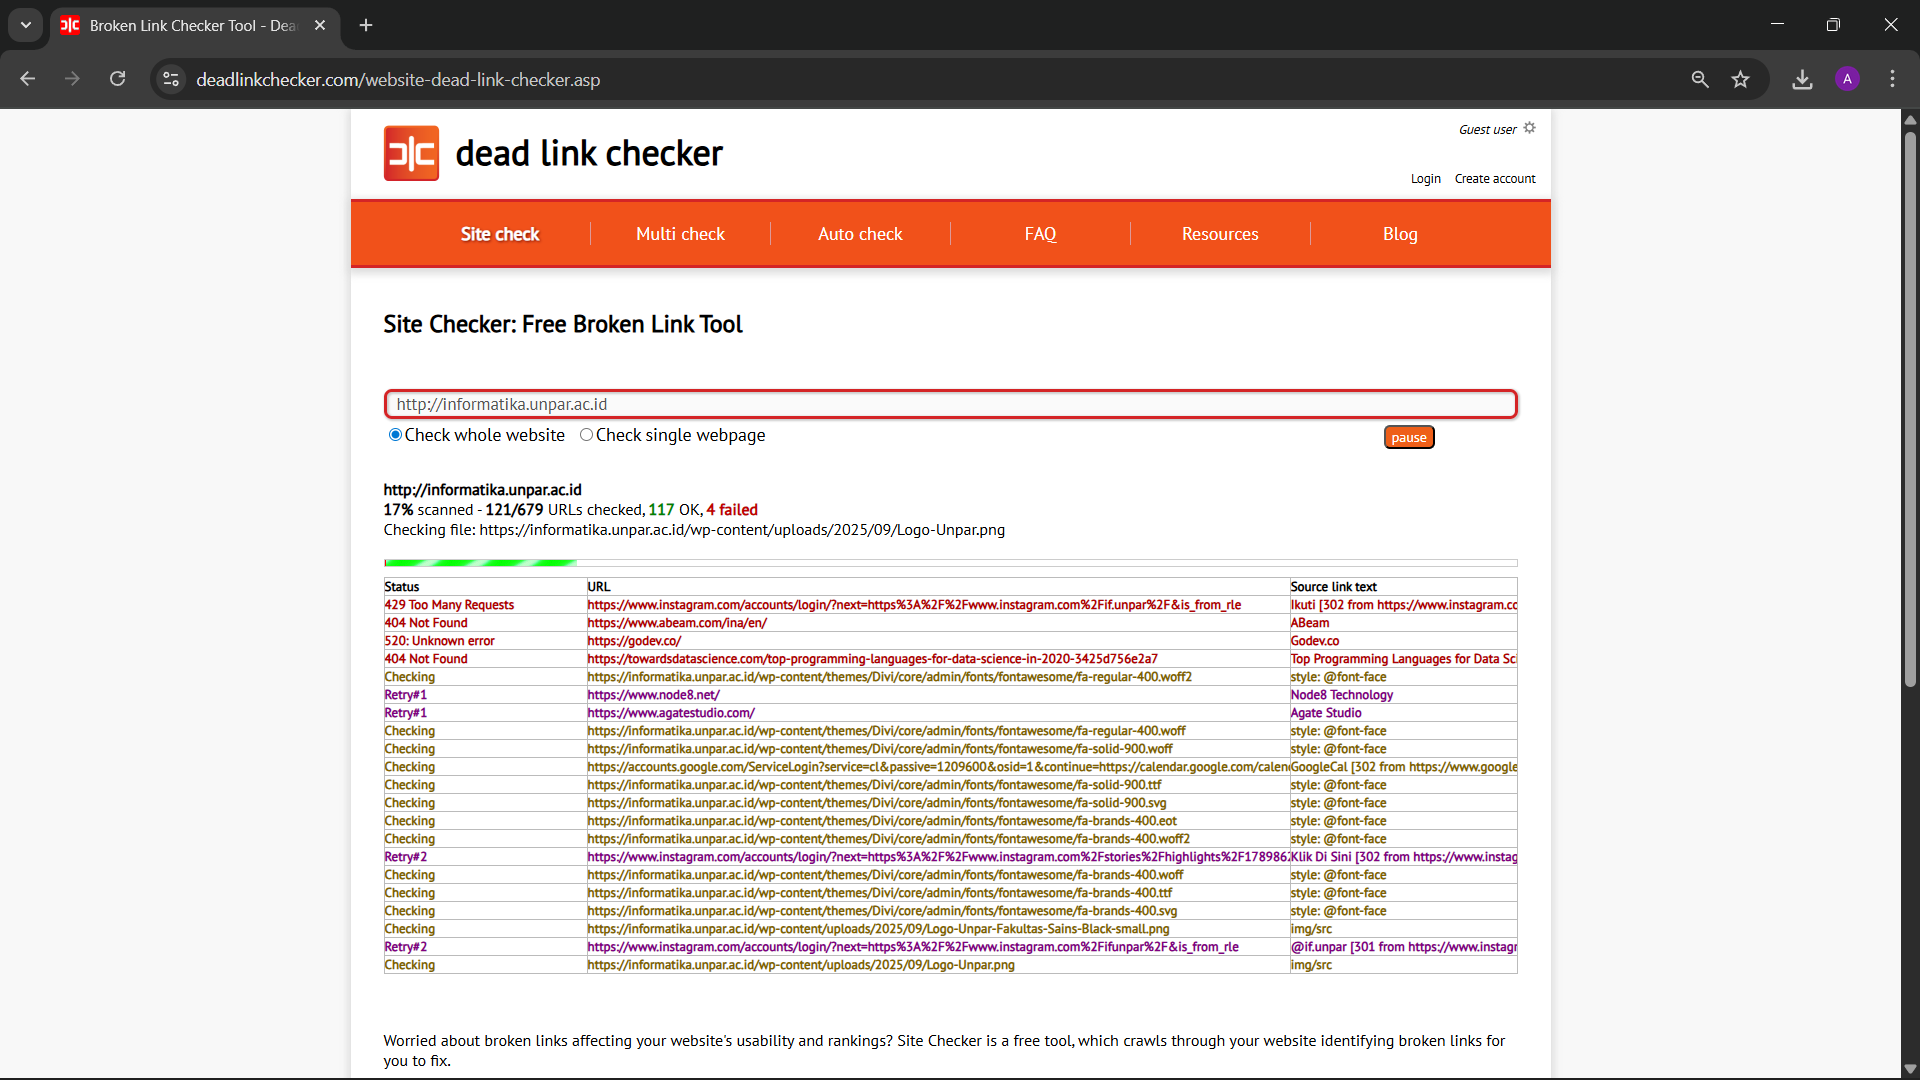
\includegraphics[width=0.9\textwidth]{Gambar/030202-dead-link-checker.png}
    \caption{Antarmuka Dead Link Checker}
    \label{fig:analisis-deadlinkchecker}
\end{figure}

Berikut adalah penjelasan komponen antarmuka pengguna pada layanan \textit{site check} :
\begin{enumerate}
    \item \textbf{Input URL}\\  
    Pengguna cukup memasukkan alamat domain atau halaman dengan URL absolut yang ingin diperiksa. Jika skema tidak dituliskan, sistem secara otomatis menambahkan awalan \texttt{http://}. Hal ini menyederhanakan input, meskipun dapat menimbulkan masalah pada situs yang hanya mendukung skema HTTPS.  

    \item \textbf{Mode pemeriksaan}\\  
    Dead Link Checker menyediakan dua opsi, yakni \textit{Check whole website} untuk menelusuri seluruh halaman dalam domain yang sama dengan URL input, dan \textit{Check single webpage} untuk memeriksa hanya halaman yang diberikan sesuai URL input.
 
    \item \textbf{Kontrol proses}\\
    Pemeriksaan tautan dijalankan dengan menekan tombol \textit{check}. Setelah proses berlangsung, tombol ini berubah menjadi \textit{pause} yang jika ditekan maka akan menghentikan sementara proses pemeriksaan dan menyimpan posisi terakhir. Pada kondisi jeda, tombol \textit{pause} akan digantikan dengan dua tombol, yaitu \textit{resume} untuk melanjutkan pemeriksaan dari titik terakhir, dan \textit{cancel} untuk membatalkan seluruh proses.

    \item \textbf{Ringkasan pemeriksaan}\\  
    Ringkasan pemeriksaan menampilkan informasi utama terkait progres yang sedang berlangsung. Bagian ini memuat alamat situs yang diperiksa, persentase pemindaian yang telah selesai, jumlah tautan yang sudah diperiksa dibandingkan dengan total tautan yang ditemukan, serta jumlah tautan yang berstatus OK dan yang \textit{failed}. Informasi tambahan juga ditampilkan berupa alamat tautan yang sedang diperiksa pada saat itu. Tepat di bawahnya terdapat \textit{progress bar} berwarna, di mana warna hijau beraksen putih menunjukkan jumlah tautan yang berstatus OK dan sedang di proses, sedangkan warna merah menunjukkan jumlah tautan yang gagal diakses.

    \item \textbf{Tabel hasil}\\
    Hasil pemeriksaan ditampilkan dalam bentuk tabel dengan tiga kolom utama yang isinya diperbarui secara langsung (\textit{real time}) selama pemeriksaan berlangsung. Tautan yang valid dihapus otomatis dari tabel setelah berhasil diperiksa, sehingga yang tersisa hanya entri yang bermasalah atau sedang diproses. Berikut adalah penjelasan untuk tiap kolom:
    \begin{itemize}
    
        \item \textbf{Status}: Pada kolom ini, awalnya semua tautan diberi status \textit{Checking}, jika pada tahap ini terjadi kegagalan koneksi atau tidak ada respons dari server, sistem secara otomatis melakukan percobaan ulang yang ditandai dengan \textit{Retry\#1} dan \textit{Retry\#2}. Apabila setelah dua kali percobaan ulang tautan tetap tidak dapat diakses, maka status akhir ditetapkan sesuai kondisi terakhir, seperti \texttt{Timeout} atau \texttt{Host not found}. Sebaliknya, jika server memberikan respons yang jelas, sistem langsung menampilkan kode hasil tanpa melakukan retry, seperti \texttt{404 Not Found}, \texttt{500 Internal Server Error}, \texttt{429 Too Many Requests}, atau kode non-standar seperti \texttt{999}. Warna latar baris juga digunakan untuk memperjelas status: kuning untuk \textit{Checking}, ungu untuk \textit{Retry}, dan merah untuk tautan yang rusak.
        
        \item \textbf{URL}: Kolom ini berisi alamat tautan yang sedang atau sudah diperiksa. Setiap entri dapat diklik untuk membuka alamat tersebut secara langsung di \textit{browser}.
        
        \item \textbf{Source link text}: Kolom ini menunjukkan teks jangkar dari tautan atau konteks halaman sumber tempat tautan ditemukan. Bagian ini juga dapat diklik untuk membuka halaman asal tautan ditemukan.
        
    \end{itemize}
\end{enumerate}

\subsubsection*{Mekanisme dan Ketentuan Teknis}  
Selain fitur yang terlihat pada antarmuka, Dead Link Checker juga memiliki mekanisme dan ketentuan teknis berikut:

\begin{enumerate}
    \item \textbf{\textit{Crawling} rekursif}\\
    Dead Link Checker bekerja dengan cara \textit{crawling} halaman web secara rekursif, yaitu dengan mengikuti setiap tautan yang ditemukan untuk kemudian dipindai kembali. Proses dimulai dari URL awal, lalu setiap tautan dalam domain yang sama diperiksa dan jika valid akan diperlakukan sebagai halaman baru untuk dianalisis. Pola ini terus diulangi hingga batas kedalaman tertentu, di mana pemeriksaan penuh (\textit{full scan}) dapat menjangkau hingga sepuluh tingkat halaman. 

    \item \textbf{Kepatuhan terhadap Robots.txt}\\
    Dead Link Checker melakukan pemindaian dengan tetap menghormati aturan pada berkas \texttt{robots.txt} yang dimiliki oleh situs web target. Pada berkas ini, administrator situs dapat menentukan direktori yang tidak boleh diakses oleh crawler atau memberi jeda antar permintaan untuk mengurangi beban server. Dead Link Checker menggunakan \textit{user-agent} khusus \texttt{www.deadlinkchecker.com}, sehingga aturan yang ditulis dengan user-agent ini akan dipatuhi. Contoh aturan yang dapat ditambahkan adalah:
    
\begin{verbatim}
User-agent: www.deadlinkchecker.com
Disallow: /shoppingbasket/
Crawl-delay: 1
\end{verbatim}

    Instruksi tersebut akan mencegah \textit{crawler} mengakses direktori \texttt{/shoppingbasket/} beserta subdirektorinya, serta memaksa jeda minimal satu detik antar permintaan. Dengan mekanisme ini, pemilik situs web memiliki kendali untuk membatasi sejauh mana Dead Link Checker dapat melakukan \textit{crawling} pada situs web mereka.

\end{enumerate}



\subsection{Broken Link Checker}
\label{subsec:0302-broken-link-checker}
Broken Link Checker\footnote{\url{https://www.brokenlinkcheck.com} (Diakses pada 30 Agustus 2025)} adalah sebuah situs web yang digunakan untuk mendeteksi tautan rusak, baik tautan internal maupun eksternal pada sebuah situs web.


\subsubsection*{Tampilan dan Interaksi}

Gambar~\ref{fig:analisis-brokenlinkchecker} menunjukkan antarmuka Broken Link Checker saat proses pemeriksaan berlangsung. Alur penggunaan secara umum dimulai dengan memasukkan alamat situs pada kolom input, mengisi kode keamanan, memilih mode pemeriksaan, lalu menekan tombol \textit{Find broken links now!} untuk memulai proses. Selama pemeriksaan berjalan, hasil ditampilkan langsung dalam bentuk tabel, dan pengguna dapat menghentikan proses dengan menekan tombol \textit{Stop}.

\begin{figure}[H]
    \centering
    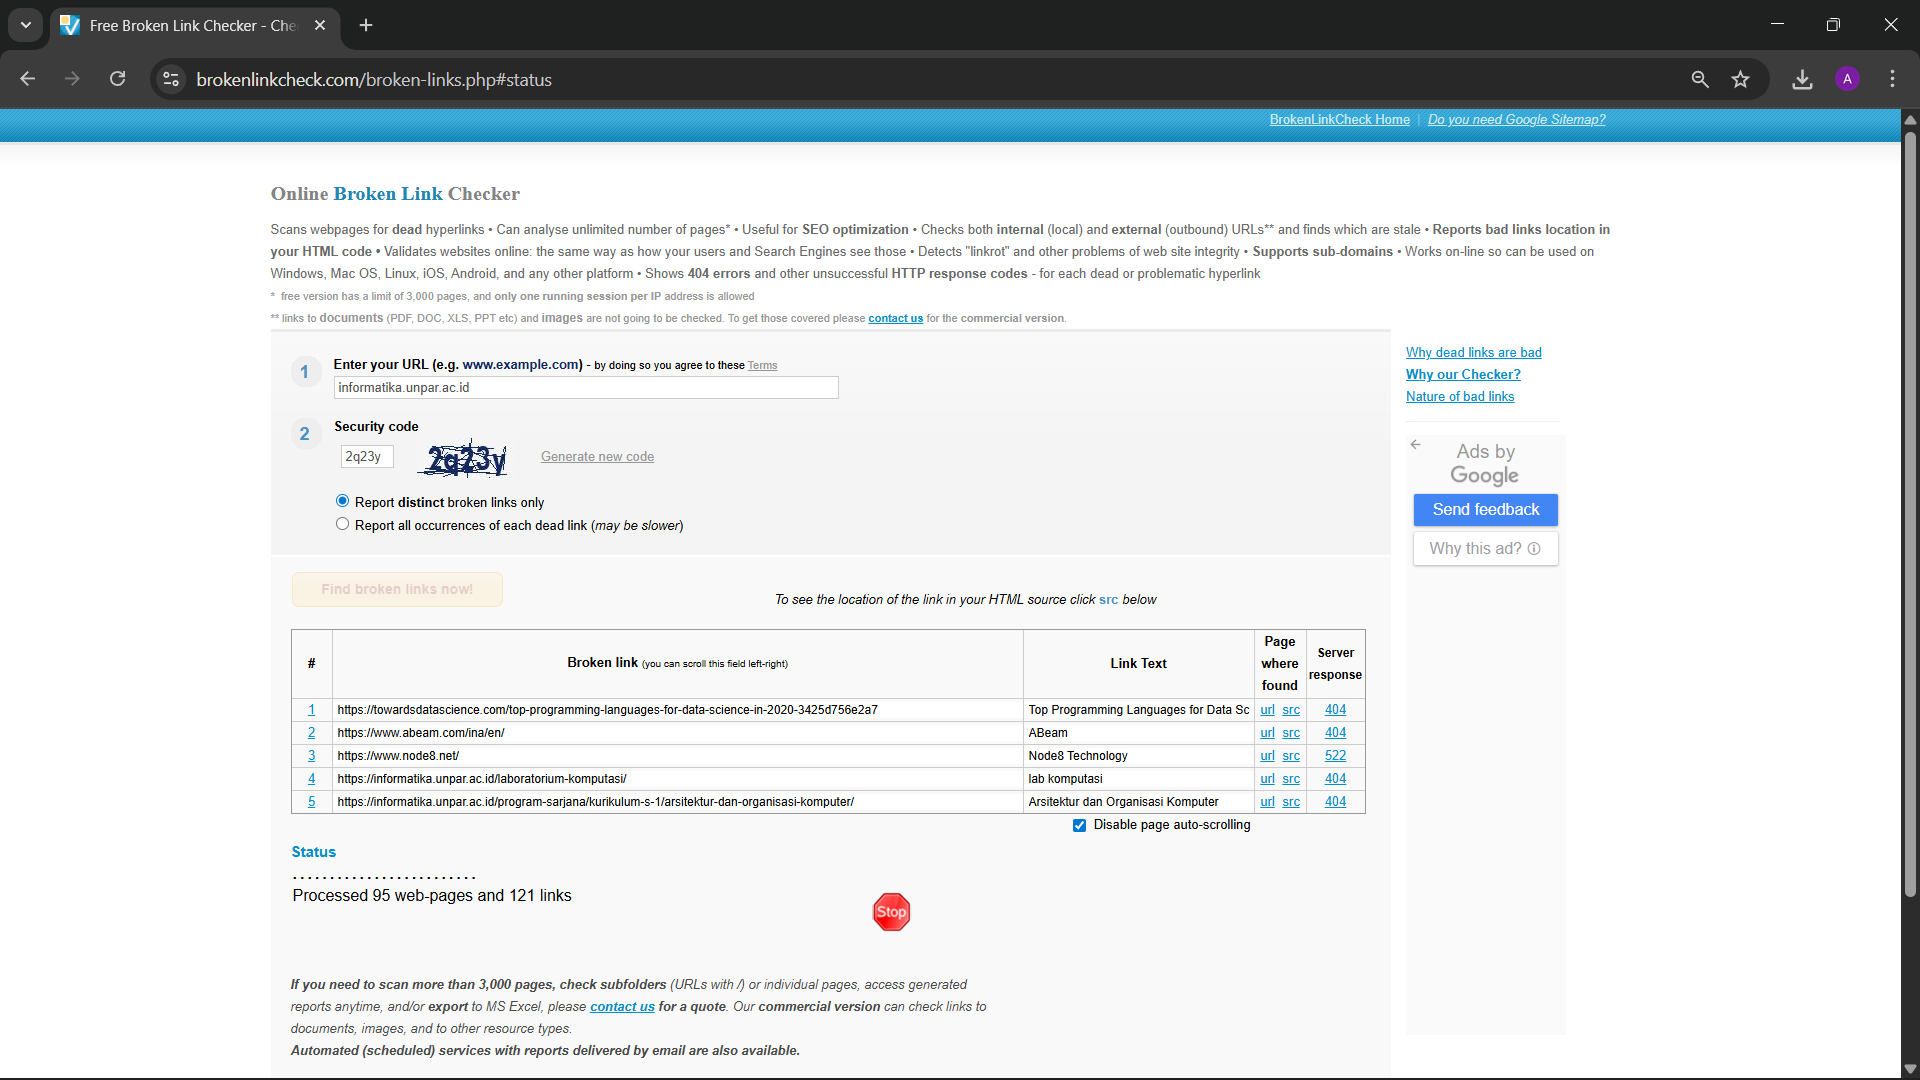
\includegraphics[width=0.95\textwidth]{Gambar/030203-broken-link-checker.png}
    \caption{Antarmuka Broken Link Checker}
    \label{fig:analisis-brokenlinkchecker}
\end{figure}

Berikut adalah komponen utama antarmuka pengguna Broken Link Checker pada layanan pemeriksaan tautan rusak:

\begin{enumerate}
    \item \textbf{Input URL}\\
    Komponen ini digunakan untuk memasukkan alamat situs web yang akan diperiksa. Pengguna dapat menuliskan alamat dalam bentuk domain saja, tanpa harus menyertakan skema \texttt{http://} atau \texttt{https://}. Sistem akan tetap menerima input tersebut dan mengolahnya sebagai URL awal pemeriksaan. Kemudahan ini mempersingkat proses input, meskipun dapat menimbulkan potensi ambiguitas pada situs web yang hanya mendukung skema tertentu, misalnya hanya \texttt{https://}.

    \item \textbf{Security code}\\
    Sebelum memulai proses pemeriksaan, pengguna diwajibkan mengisi \textit{security code} berupa captcha. Keharusan ini berfungsi sebagai mekanisme pencegahan terhadap penggunaan otomatis (bot) yang dapat membebani server layanan. Kode keamanan ini bersifat dinamis dan dapat diganti dengan menekan tombol \textit{Generate new code} yang tersedia pada antarmuka.

    \item \textbf{Mode pemeriksaan}\\
    Tersedia dua pilihan mode pemeriksaan yang dapat dipilih melalui tombol radio, yaitu \textit{Report distinct broken links only}, dan \textit{Report all occurrences of each dead link}. Mode \textit{Report distinct broken links only} menampilkan setiap tautan rusak hanya sekali, tanpa memperhatikan berapa banyak halaman yang memuat tautan tersebut. Pendekatan ini membuat proses lebih cepat, tetapi informasi lokasi kemunculan tautan hanya terbatas pada satu halaman. Sebaliknya, mode \textit{Report all occurrences of each dead link (may be slower)} menampilkan seluruh kemunculan tautan rusak beserta halaman sumbernya. Dengan demikian, jika sebuah tautan rusak terdapat pada beberapa halaman, maka akan muncul beberapa entri dengan sumber berbeda pada tabel hasil. Mode ini memberikan informasi yang lebih lengkap, namun membutuhkan waktu pemrosesan yang lebih lama.

    \item \textbf{Tombol kontrol}\\
    Proses pemeriksaan dimulai dengan menekan tombol \textit{Find broken links now!}. Setelah pemeriksaan berjalan, tombol \textit{Stop} berwarna merah akan muncul di bawah tabel hasil. Tombol ini memungkinkan pengguna menghentikan proses pemeriksaan kapan saja sesuai kebutuhan. Selain itu, disediakan pula opsi \textit{Disable page auto-scrolling} yang dapat diaktifkan untuk menonaktifkan pengguliran otomatis pada tabel hasil, sehingga tampilan tetap stabil meskipun data baru terus ditambahkan secara real-time.

    \item \textbf{Tabel hasil}\\
    Hasil pemeriksaan ditampilkan dalam bentuk tabel yang diperbarui secara langsung. Tabel ini hanya menampilkan tautan yang telah dipastikan bermasalah, sehingga laporan lebih fokus dan tidak bercampur dengan tautan valid atau sedang dalam proses pemeriksaan. Terdapat lima kolom utama pada tabel hasil, yaitu:
    
    \begin{itemize}
    
        \item \textbf{\#}: kolom nomor urut hasil. Setiap nomor dapat diklik untuk membuka tautan rusak yang bersangkutan secara langsung.
        
        \item \textbf{Broken link}: berisi alamat tautan yang teridentifikasi rusak. Tautan ini ditampilkan dalam bentuk teks biasa tanpa fungsi klik.
        
        \item \textbf{Link text}: menampilkan teks jangkar (\textit{anchor text}) dari tautan yang ditemukan, atau keterangan terkait jika tersedia.
        
        \item \textbf{Page where found}: berisi dua tautan, yaitu \textit{url} yang mengarah ke halaman web tempat tautan rusak ditemukan, serta \textit{src} yang menunjuk ke dokumen HTML sumber untuk memperlihatkan lokasi tautan yang bermasalah.
        
        \item \textbf{Server response}: menampilkan status akhir dari hasil pemeriksaan tautan, baik berupa kode status HTTP seperti \texttt{404} dan \texttt{500}, maupun pesan kesalahan non-HTTP seperti \texttt{bad host} atau \texttt{timeout}.
        
    \end{itemize}

    \item \textbf{Ringkasan pemeriksaan}\\
    Pada bagian bawah tabel, sistem menampilkan ringkasan proses pemeriksaan yang sedang berlangsung. Bagian ini memuat status terkini, yang ditandai dengan animasi titik berjalan selama proses aktif. Jika pemeriksaan dihentikan oleh pengguna melalui tombol \textit{Stop}, status akan berubah menjadi \texttt{DONE : process was terminated by user}. Sebaliknya, jika pemeriksaan selesai secara normal, status ditampilkan sebagai \texttt{COMPLETED!}. Selain menampilkan status, ringkasan ini juga memperlihatkan jumlah total halaman dan tautan yang telah diperiksa, serta jumlah tautan rusak yang ditemukan.
\end{enumerate}


\subsubsection*{Mekanisme dan Ketentuan Teknis}  
Selain fitur yang tampak pada antarmuka, Broken Link Checker juga memiliki sejumlah mekanisme teknis yang menentukan cara kerja dan batasan layanan. Mekanisme ini penting untuk dipahami agar pengguna dapat menafsirkan hasil pemeriksaan dengan tepat dan menyesuaikan penggunaan sesuai kebutuhan. Mekanisme dan ketentuan teknis tersebut dapat dirangkum sebagai berikut:

\begin{enumerate}
    \item \textbf{Cakupan pemeriksaan}\\
    Broken Link Checker melakukan pemeriksaan terhadap tautan internal maupun eksternal dari sebuah situs web. Tautan internal adalah tautan yang berada dalam domain yang sama dengan URL awal, sedangkan tautan eksternal adalah tautan yang mengarah keluar ke domain lain. Hanya tautan yang bermasalah yang ditampilkan dalam laporan, sedangkan tautan valid tidak ditampilkan. Pendekatan ini membuat hasil pemeriksaan lebih bersih dan mudah dianalisis karena pengguna tidak perlu memilah-milah tautan yang sebenarnya masih berfungsi.

    \item \textbf{Batasan versi gratis}\\
    Versi gratis dari layanan ini memiliki beberapa pembatasan. Pemeriksaan hanya dapat dilakukan hingga maksimum 3.000 halaman dalam satu sesi, dengan ketentuan satu sesi diperbolehkan untuk setiap alamat IP pada satu waktu. Selain itu, pemeriksaan pada versi gratis tidak mencakup tautan yang menuju ke dokumen seperti PDF, DOC, XLS, PPT, maupun tautan ke file gambar. Batasan ini diberlakukan untuk mengurangi beban layanan sekaligus mendorong pengguna yang membutuhkan cakupan lebih luas untuk beralih ke versi komersial.

    \item \textbf{Fitur versi komersial}\\
    Untuk kebutuhan yang lebih kompleks, Broken Link Checker menyediakan layanan berbayar dengan fitur tambahan. Pada versi ini, pemeriksaan dapat dilakukan pada jumlah halaman yang jauh lebih besar tanpa batasan ketat seperti pada versi gratis. Selain itu, layanan berbayar mendukung pemindaian sub-folder dan sub-domain, pemeriksaan tautan yang mengarah ke dokumen maupun gambar, serta ekspor hasil pemeriksaan ke format CSV atau Excel untuk memudahkan analisis lanjutan. Fitur lain yang ditawarkan mencakup pembuatan laporan otomatis yang dikirim melalui email secara terjadwal (harian, mingguan, atau bulanan), opsi konfigurasi kecepatan pemeriksaan sesuai kebutuhan situs target, serta analisis tambahan seperti pemeriksaan feed RSS atau ATOM.
\end{enumerate}



\section{Analisis Kebutuhan}
\label{sec:03-analisis-kebutuhan}
% 


Analisis masalah pada Subbab~\ref{sec:03-analisis-masalah}, serta analisis sistem serupa pada Subbab~\ref{sec:03-analisis-sistem-serupa}, menghasilkan gambaran mengenai fitur dan karakteristik yang harus dimiliki oleh sistem. Dari sini disusun kebutuhan fungsional yang menjelaskan layanan apa saja yang harus disediakan oleh sistem, serta kebutuhan non-fungsional yang berhubungan dengan kualitas, batasan teknis, dan kriteria pendukung lainnya.


\subsection{Kebutuhan Fungsional}
\label{subsec:0303-kebutuhan-fungsional}

Kebutuhan fungsional berikut menggambarkan layanan inti yang harus disediakan oleh aplikasi desktop pemeriksa tautan rusak pada situs web:

\begin{enumerate}
    \item \textbf{Input URL}\\
    Sistem harus dapat menerima masukan berupa URL dari pengguna sebagai titik awal pemeriksaan.

    \item \textbf{Tampilan hasil secara \textit{streaming}}\\
    Sistem menampilkan daftar tautan yang ditemukan dari halaman web secara langsung (\textit{streaming}) selama proses pemeriksaan berlangsung.

    \item \textbf{Penghentian proses}\\
    Sistem menyediakan mekanisme bagi pengguna untuk menghentikan proses pemeriksaan kapan saja.

    \item \textbf{Mekanisme \textit{retry}}\\
    Sistem melakukan percobaan ulang terhadap tautan yang gagal diperiksa akibat kesalahan sementara, misalnya \textit{timeout} atau gangguan jaringan.

    \item \textbf{Ringkasan hasil}\\
    sistem menampilkan ringkasan berisi jumlah tautan yang diperiksa, jumlah tautan rusak, jumlah tautan yang terblokir, dan status proses pemeriksaan.


    \item \textbf{Sumber tautan rusak}\\
    Sistem menampilkan lokasi atau halaman tempat tautan rusak ditemukan, sehingga pengguna dapat menelusuri asal masalah.

    \item \textbf{Ekspor hasil}\\
    Sistem dapat mengekspor hasil pemeriksaan ke dalam berkas Excel agar mudah disimpan, dibagikan, atau dianalisis lebih lanjut.
\end{enumerate}


\subsection{Kebutuhan Non-Fungsional}
\label{subsec:0303-kebutuhan-non-fungsional}

Selain fungsi inti, sistem juga harus memenuhi sejumlah kebutuhan non-fungsional agar pemeriksaan tautan dapat berjalan stabil, efisien, dan mudah digunakan. Kebutuhan non-fungsional yang ditetapkan adalah sebagai berikut:

\begin{enumerate}
    \item \textbf{Antarmuka pengguna}\\
    Sistem disajikan dalam bentuk aplikasi desktop berbasis JavaFX dengan tampilan yang sederhana, tabel yang mudah dibaca, serta kontrol proses yang jelas.

    \item \textbf{Kinerja pemeriksaan}\\
    Sistem mampu menangani jumlah tautan yang besar dengan tetap menjaga waktu tanggap yang wajar. Hal ini dicapai dengan penerapan batas waktu (\textit{timeout}) pada setiap permintaan.

    \item \textbf{Pengendalian laju}\\
    Sistem membatasi jumlah permintaan dalam satuan waktu (\textit{rate limiting}) untuk mencegah server tujuan terbebani dan mengurangi risiko pemblokiran.

    \item \textbf{Eksekusi paralel}\\
    Sistem mendukung eksekusi permintaan secara paralel (\textit{concurrency}) khusus pada tahap pemeriksaan tautan agar proses lebih cepat. Jumlah permintaan simultan dibatasi agar tetap stabil dan tidak menimbulkan masalah \texttt{429 Too Many Requests} atau pemblokiran.

    \item \textbf{Ketahanan terhadap HTML tidak valid}\\
    Sistem mampu mengurai dokumen HTML yang tidak sesuai standar dengan bantuan Jsoup, sehingga tautan tetap dapat diekstrak meskipun struktur dokumen bermasalah.

    \item \textbf{Konsistensi identifikasi URL}\\
    Setiap URL dinormalisasi dan dicatat dalam repository untuk memastikan satu sumber daya hanya diperiksa sekali, sehingga hasil pemeriksaan konsisten dan tidak ada duplikasi.

    \item \textbf{Pelabelan hasil yang jelas}\\
    Setiap hasil pemeriksaan ditampilkan dengan kode status HTTP beserta keterangan resminya, serta pesan khusus untuk kesalahan non-HTTP seperti \textit{timeout}, \textit{bad host}, atau kesalahan koneksi.

    \item \textbf{Etika \textit{crawling}}\\
    Setiap permintaan menyertakan identitas \texttt{User-Agent}. Sistem juga menyediakan pengaturan jeda permintaan untuk menjaga agar aktivitas pemeriksaan tidak membebani server.

\end{enumerate}



\section{Analisis Teknologi yang Digunakan}
\label{sec:03-analisis-teknologi-yang-digunakan}
% % \subsection{Gradle}
% \label{subsec:0304-gradle}
% 
Gradle merupakan sistem otomasi pembangunan perangkat lunak (\textit{build automation}) yang digunakan untuk mengelola proses kompilasi, pengujian, dan distribusi perangkat lunak. Gradle dikembangkan sebagai generasi lanjutan dari sistem build sebelumnya seperti Apache Ant dan Maven, dengan tujuan menyediakan mekanisme yang lebih fleksibel dan dapat diprogram.  

Gradle menggunakan \textit{domain-specific language} (DSL) berbasis Groovy atau Kotlin untuk mendefinisikan proses build. Pendekatan ini menggabungkan gaya deklaratif, di mana pengembang menyatakan konfigurasi yang diinginkan, dengan gaya imperatif, di mana logika tambahan dapat ditulis sebagai kode program. Dengan demikian, Gradle memungkinkan penulisan skrip build yang ringkas namun tetap mendukung kustomisasi tingkat lanjut.  

Arsitektur Gradle didesain modular dan berbasis plugin. Plugin menyediakan konfigurasi dan sekumpulan \textit{task} standar sesuai kebutuhan proyek, misalnya untuk membangun aplikasi Java atau mengelola arsip distribusi. Sistem ini juga terintegrasi dengan repositori perangkat lunak seperti Maven Central, sehingga dependensi eksternal dapat diunduh dan dikelola secara otomatis.

\subsection{Konsep Build dan Task}
Dalam pengembangan perangkat lunak, proses \textit{build} mencakup serangkaian langkah seperti kompilasi kode sumber, manajemen dependensi, pengujian otomatis, serta pembuatan artefak distribusi seperti JAR atau WAR. Gradle memodelkan setiap langkah tersebut sebagai \textit{task}, yaitu unit kerja terpisah yang dapat dijalankan secara independen maupun sebagai bagian dari rangkaian tugas lain.  

Setiap task memiliki tindakan utama (\textit{action}) dan dapat didefinisikan dengan ketergantungan terhadap task lain. Dengan cara ini, Gradle membangun sebuah grafik ketergantungan yang menentukan urutan eksekusi seluruh proses build.  

Kode~\ref{lst:gradle-simple-task} memperlihatkan contoh definisi task sederhana dalam Gradle.

\begin{lstlisting}[language=groovy, caption=Contoh task sederhana dalam Gradle, label=lst:gradle-simple-task]
task cetakPesan {
    doLast {
        println 'Ini adalah task pertama saya di Gradle!'
    }
}
\end{lstlisting}

Kode pada Kode~\ref{lst:gradle-simple-task} mendefinisikan sebuah task bernama \texttt{cetakPesan}. Task ini memiliki satu aksi yang dijalankan pada fase \texttt{doLast}, yaitu mencetak pesan ke konsol. Task dapat dijalankan secara langsung dengan perintah \texttt{gradle cetakPesan}, dan Gradle akan mengeksekusi instruksi yang terdefinisi di dalamnya. Dengan pendekatan ini, pengembang dapat mendefinisikan berbagai tahapan build secara modular dan dapat digunakan kembali.


\subsection{Struktur Proyek}
Gradle mendukung struktur proyek yang fleksibel, tetapi umumnya mengikuti konvensi tertentu agar proses build lebih sederhana. Beberapa berkas dan direktori yang umum ditemukan dalam proyek Gradle antara lain:  

\begin{itemize}
    \item \texttt{build.gradle}, berisi deklarasi task, konfigurasi plugin, dan daftar dependensi.
    \item \texttt{settings.gradle}, mendefinisikan nama proyek dan konfigurasi multiproject bila proyek terdiri dari lebih dari satu modul.
    \item \texttt{src/main/java}, direktori utama untuk kode sumber aplikasi Java.
    \item \texttt{src/test/java}, direktori untuk kode pengujian unit.
\end{itemize}

Kode~\ref{lst:gradle-java} memperlihatkan contoh berkas \texttt{build.gradle} untuk proyek Java sederhana.

\begin{lstlisting}[language=groovy, caption=Contoh berkas build.gradle untuk proyek Java, label=lst:gradle-java]
plugins {
    id 'java'
    id 'application'
}

repositories {
    mavenCentral()
}

dependencies {
    implementation 'org.jsoup:jsoup:1.15.4'
    testImplementation 'junit:junit:4.13.2'
}

application {
    mainModule = 'com.unpar.brokenlinkchecker'
    mainClass = 'com.unpar.brokenlinkchecker.Application'
}
\end{lstlisting}

Kode pada Kode~\ref{lst:gradle-java} menunjukkan bagaimana proyek Java didefinisikan dalam Gradle. Pada bagian \texttt{plugins}, diaktifkan plugin \texttt{java} untuk mendukung kompilasi kode Java dan plugin \texttt{application} untuk menjalankan aplikasi. Bagian \texttt{repositories} menentukan bahwa dependensi diambil dari \texttt{mavenCentral}. Selanjutnya, blok \texttt{dependencies} mendefinisikan pustaka eksternal yang digunakan, yaitu \texttt{jsoup} untuk pemrosesan HTML dan \texttt{junit} untuk pengujian. Pada blok \texttt{application}, ditentukan modul utama dan kelas utama yang menjadi titik masuk aplikasi.


\subsection{Struktur Proyek}
Gradle mendukung struktur proyek yang fleksibel, tetapi umumnya mengikuti konvensi tertentu agar proses build lebih sederhana. Beberapa berkas dan direktori yang umum ditemukan dalam proyek Gradle antara lain:  

\begin{itemize}
    \item \texttt{build.gradle}, berisi deklarasi task, konfigurasi plugin, dan daftar dependensi.
    \item \texttt{settings.gradle}, mendefinisikan nama proyek dan konfigurasi multiproject bila proyek terdiri dari lebih dari satu modul.
    \item \texttt{src/main/java}, direktori utama untuk kode sumber aplikasi Java.
    \item \texttt{src/test/java}, direktori untuk kode pengujian unit.
\end{itemize}

Kode~\ref{lst:gradle-java} memperlihatkan contoh berkas \texttt{build.gradle} untuk proyek Java sederhana.

\begin{lstlisting}[language=groovy, caption=Contoh berkas build.gradle untuk proyek Java, label=lst:gradle-java]
plugins {
    id 'java'
    id 'application'
}

repositories {
    mavenCentral()
}

dependencies {
    implementation 'org.jsoup:jsoup:1.15.4'
    testImplementation 'junit:junit:4.13.2'
}

application {
    mainModule = 'com.unpar.brokenlinkchecker'
    mainClass = 'com.unpar.brokenlinkchecker.Application'
}
\end{lstlisting}

Kode pada Kode~\ref{lst:gradle-java} menunjukkan bagaimana proyek Java didefinisikan dalam Gradle. Pada bagian \texttt{plugins}, diaktifkan plugin \texttt{java} untuk mendukung kompilasi kode Java dan plugin \texttt{application} untuk menjalankan aplikasi. Bagian \texttt{repositories} menentukan bahwa dependensi diambil dari \texttt{mavenCentral}. Selanjutnya, blok \texttt{dependencies} mendefinisikan pustaka eksternal yang digunakan, yaitu \texttt{jsoup} untuk pemrosesan HTML dan \texttt{junit} untuk pengujian. Pada blok \texttt{application}, ditentukan modul utama dan kelas utama yang menjadi titik masuk aplikasi.


\subsection{Plugin, Repositori, dan DSL}
Gradle memiliki arsitektur berbasis plugin. Plugin menyediakan konfigurasi dan sekumpulan task yang sesuai dengan jenis proyek tertentu. Sebagai contoh, plugin \texttt{java} menambahkan task untuk kompilasi dan pengujian kode Java, sedangkan plugin \texttt{application} menambahkan task untuk menjalankan aplikasi.  

Dependensi eksternal dikelola melalui sistem repositori. Gradle mendukung berbagai repositori seperti \texttt{mavenCentral}, \texttt{jcenter}, maupun repositori lokal. Dengan pendekatan ini, pustaka pihak ketiga dapat diunduh secara otomatis dan disertakan dalam proses build.  

Gradle menggunakan \textit{domain-specific language} (DSL) berbasis Groovy atau Kotlin untuk menuliskan konfigurasi build. DSL ini memungkinkan pengembang mendefinisikan task, plugin, repositori, dan dependensi dalam bentuk blok kode yang ringkas. Konsep seperti \textit{closure} dan \textit{convention-over-configuration} digunakan untuk menyederhanakan sintaks sekaligus tetap memberikan fleksibilitas dalam kustomisasi alur build.


\subsection{Siklus Eksekusi Gradle}
Proses eksekusi build pada Gradle berlangsung dalam dua fase utama, yaitu fase konfigurasi dan fase eksekusi.  

Pada fase konfigurasi, Gradle membaca seluruh berkas skrip build seperti \texttt{build.gradle} dan \texttt{settings.gradle}. Seluruh definisi task, plugin, dan konfigurasi dievaluasi untuk membangun model tugas beserta ketergantungan antar tugas. Pada tahap ini belum ada task yang dijalankan, melainkan hanya persiapan struktur eksekusi.  

Setelah konfigurasi selesai, Gradle memasuki fase eksekusi. Pada tahap ini, Gradle menjalankan task yang diminta beserta seluruh dependensinya sesuai dengan urutan yang telah ditentukan. Fase eksekusi memastikan setiap task dijalankan satu kali dan hanya jika dibutuhkan, misalnya saat terjadi perubahan pada kode sumber.  

Pemisahan yang jelas antara fase konfigurasi dan fase eksekusi memungkinkan Gradle mengelola alur build secara efisien dan fleksibel, serta memberikan kendali penuh kepada pengembang dalam menuliskan logika build.


\subsection{JavaFX}
\label{subsec:0304-javafx}
% \subsection{JavaFX}
% \label{subsec:0304-javafx}

Pemilihan JavaFX sebagai pustaka antarmuka pengguna didasarkan pada kebutuhan sistem yang harus disajikan dalam bentuk aplikasi desktop dengan tampilan sederhana, tabel yang mudah dibaca, serta kontrol proses yang jelas (lihat Subsubbab~\ref{subsec:0303-kebutuhan-non-fungsional}). Sebagaimana dijelaskan pada Subbab~\ref{sec:02-javafx}, JavaFX menawarkan paradigma \textit{scene graph} yang memungkinkan penyusunan antarmuka secara hierarkis dan konsisten. Paradigma ini memudahkan pengelolaan komponen visual yang diperlukan untuk menampilkan hasil pemeriksaan tautan secara \textit{streaming} (lihat Subsubbab~\ref{subsec:0303-kebutuhan-fungsional}).

Dalam implementasi, JavaFX akan digunakan melalui beberapa komponen utama berikut:

\begin{itemize}
  \item \textbf{Stage, Scene, dan Node}. Struktur dasar aplikasi akan mengikuti siklus hidup JavaFX dengan menurunkan kelas dari \texttt{Application}. Objek \texttt{Stage} akan berperan sebagai jendela utama, sedangkan \texttt{Scene} digunakan untuk menampung keseluruhan antarmuka. Komponen UI seperti \texttt{Button}, \texttt{Label}, dan \texttt{TextField} direpresentasikan sebagai turunan \texttt{Node} yang diorganisasi dalam kontainer tata letak, misalnya \texttt{VBox} atau \texttt{BorderPane}.

  \item \textbf{FXML dan Controller}. Untuk memisahkan logika aplikasi dari tampilan, struktur antarmuka didefinisikan secara deklaratif dalam berkas FXML. Atribut \texttt{fx:id} akan dipakai agar komponen UI dapat diakses dari kelas controller, sedangkan event handler seperti \texttt{onAction} digunakan untuk menangani interaksi pengguna, misalnya saat memulai atau menghentikan proses pemeriksaan tautan.

  \item \textbf{Komponen Tabel}. Hasil pemeriksaan tautan akan ditampilkan dalam bentuk tabel menggunakan \texttt{TableView}. Komponen ini mendukung penyajian data terstruktur dalam baris dan kolom, sehingga cocok untuk menampilkan daftar halaman yang diperiksa maupun daftar tautan rusak. Setiap kolom akan diikat dengan \texttt{Property} pada model data agar perubahan nilai dapat langsung tercermin pada tampilan.

  \item \textbf{Property dan Binding}. Untuk mendukung pembaruan data secara langsung, mekanisme \texttt{StringProperty}, \texttt{BooleanProperty}, dan \texttt{IntegerProperty} akan digunakan. Binding dua arah dimanfaatkan agar nilai pada komponen input dan model selalu konsisten, sedangkan binding satu arah memastikan perubahan status pemeriksaan langsung diperlihatkan pada label atau tabel.

  \item \textbf{Pengendalian Thread}. Karena proses pemeriksaan tautan berjalan secara paralel, pembaruan antarmuka pengguna harus dijalankan melalui \texttt{Platform.runLater()}. Hal ini menjamin sinkronisasi antara \textit{thread} pemeriksaan dengan \textit{thread} JavaFX, sehingga tampilan dapat diperbarui secara aman tanpa menimbulkan error \texttt{Not on FX application thread}.
\end{itemize}



\subsection{Jsoup}
\label{subsec:0304-jsoup}
% \subsection{Jsoup}
% \label{subsec:0304-jsoup}

Pemilihan Jsoup sebagai pustaka utama untuk pengambilan dan pemrosesan dokumen HTML didasarkan pada kebutuhan sistem untuk mengekstraksi tautan dari halaman web dengan cara yang andal, termasuk dari dokumen yang tidak valid atau tidak sepenuhnya sesuai standar. Kebutuhan ini secara eksplisit dinyatakan pada aspek ketahanan terhadap HTML tidak valid (lihat Subsubbab~\ref{subsec:0303-kebutuhan-non-fungsional}). Sebagaimana dijelaskan pada Subbab~\ref{sec:02-jsoup}, Jsoup menyediakan parser yang toleran kesalahan dan mendukung spesifikasi HTML5, sehingga struktur DOM tetap dapat dibentuk meskipun dokumen bermasalah. 

Dari sisi fungsional, penggunaan Jsoup relevan dengan kebutuhan untuk:
\begin{itemize}
  \item menerima masukan URL dan mengambil halaman web terkait (lihat Subsubbab~\ref{subsec:0303-kebutuhan-fungsional}).
  \item mengekstraksi seluruh tautan yang terdapat di dalam elemen HTML, khususnya elemen \texttt{<a>} dengan atribut \texttt{href}.
  \item menampilkan hasil pemeriksaan secara \textit{streaming}, sehingga setiap tautan yang diperoleh dari hasil parsing dapat segera diperiksa dan ditampilkan ke antarmuka pengguna.
\end{itemize}

Dalam implementasi, beberapa kelas dan method dari Jsoup akan digunakan secara langsung, yaitu:

\begin{itemize}
  \item \texttt{Jsoup}\\
  Kelas ini dipakai sebagai titik masuk untuk membuat koneksi HTTP ke sebuah halaman melalui \texttt{connect(String url)}. Method ini dilanjutkan dengan konfigurasi \texttt{userAgent(String ua)} untuk memenuhi etika \textit{crawling} dan \texttt{timeout(int millis)} untuk memenuhi kebutuhan non-fungsional terkait batas waktu respon. Eksekusi permintaan dilakukan dengan \texttt{get()} atau \texttt{execute()}, menghasilkan \texttt{Document} atau \texttt{Connection.Response}.

  \item \texttt{Connection} dan \texttt{Connection.Response}\\
  \texttt{Connection} digunakan untuk mengatur parameter koneksi, sementara \texttt{Connection.Response} diperlukan untuk membaca kode status HTTP dengan \texttt{statusCode()} serta metadata lain seperti \texttt{headers()}. Informasi ini mendukung kebutuhan untuk melabeli hasil pemeriksaan dengan status yang jelas (lihat Subsubbab~\ref{subsec:0303-kebutuhan-non-fungsional}).

  \item \texttt{Document}\\
  Objek ini merepresentasikan halaman web yang berhasil diambil. Method \texttt{select(String cssQuery)} akan dipakai untuk menemukan seluruh elemen \texttt{<a>} dengan atribut \texttt{href}. Dari sini dihasilkan objek \texttt{Elements}.

  \item \texttt{Elements} dan \texttt{Element}\\
  Koleksi \texttt{Elements} berisi banyak \texttt{Element} yang masing-masing mewakili sebuah tautan. Method penting yang digunakan adalah \texttt{attr("href")} untuk mengambil nilai atribut asli, \texttt{text()} untuk isi teks tautan, serta \texttt{absUrl("href")} untuk memperoleh URL absolut berdasarkan \texttt{baseUri()} dokumen. Normalisasi URL ini mendukung konsistensi identifikasi sumber daya (lihat Subsubbab~\ref{subsec:0303-kebutuhan-non-fungsional}).

\end{itemize}


\subsection{Java HTTP Client API}
\label{subsec:0304-java-http-client-api}
Java HTTP Client API secara garis besar adalah sebuah API dari Java yang digunakan untuk mengirim \textit{request} dan menerima \textit{response} melalui protokol HTTP. API ini pertama kali diperkenalkan pada Java 9 dengan nama \texttt{jdk.incubator.httpclient} sebagai \textit{incubating module}, yaitu modul percobaan yang digunakan untuk memperkenalkan API baru sebelum akhirnya ditetapkan sebagai bagian resmi dari Java 11. Java HTTP Client API mendukung penggunaan protokol HTTP/1.1 dan HTTP/2. Secara bawaan, pemilihan versi protokol dilakukan secara otomatis, di mana \texttt{HttpClient} akan mencoba menggunakan HTTP/2 terlebih dahulu dan melakukan \textit{fallback} ke HTTP/1.1 apabila server tidak mendukung HTTP/2. Selain mekanisme bawaan tersebut, pengembang juga dapat menetapkan versi protokol secara eksplisit melalui metode yang tersedia pada kelas \texttt{HttpClient}.

Selain mendukung dua versi protokol HTTP, API ini juga menyediakan dua model komunikasi, yaitu sinkron dan asinkron. Komunikasi sinkron berarti eksekusi program akan menunggu hingga \textit{response} (\textit{response}) dari server diterima sepenuhnya sebelum melanjutkan instruksi berikutnya. Sebaliknya, komunikasi asinkron menggunakan kelas \texttt{CompletableFuture}, yang memungkinkan hasil komputasi diperoleh di masa mendatang tanpa harus menunggu proses selesai. Objek \texttt{HttpClient} dalam API ini juga memiliki karakteristik penting untuk penggunaan di lingkungan \textit{multithreaded}. Objek ini bersifat \textit{immutable}, artinya konfigurasi tidak dapat diubah setelah dibuat, serta bersifat \textit{thread-safe}, artinya dapat diakses secara bersamaan oleh beberapa \textit{thread} tanpa menimbulkan \textit{race condition}.

\subsection{\texttt{HttpClient}}
\label{subsec:0228-httpclient}

Kelas \texttt{HttpClient} merupakan komponen inti dalam Java HTTP Client API yang digunakan untuk mengirim \textit{request} HTTP dan menerima \textit{response} dari server. Objek dari kelas ini dapat dibuat dengan menggunakan \textit{static method} \texttt{newHttpClient} dengan konfigurasi bawaan yang siap pakai, atau bisa menggunakan \textit{static method} \texttt{newBuilder} apabila ingin membuat objek dengan konfigurasi yang disesuaikan.

Berikut ini adalah beberapa \textit{method} untuk menetapkan konfigurasi, yang tersedia pada objek \textit{builder} \texttt{newBuilder}:

\begin{itemize}
    \item \texttt{version}\\
    \textit{Method} ini berfungsi untuk menentukan versi protokol HTTP yang akan digunakan, yaitu \texttt{HTTP\_1\_1} atau \texttt{HTTP\_2}. Nilai yang diberikan berasal dari enum \texttt{HttpClient.Version}. Dengan pengaturan ini, klien dapat diarahkan untuk selalu memakai versi tertentu atau menyesuaikan melalui negosiasi otomatis dengan server. Pengaturan versi yang jelas membantu menjaga konsistensi komunikasi dan mencegah terjadinya ketidakcocokan protokol antara klien dan server.
    
    \item \texttt{connectTimeout}\\
    \textit{Method} ini menerima sebuah objek \texttt{Duration} yang menyatakan batas waktu maksimal dalam membangun koneksi ke server. Jika dalam jangka waktu tersebut koneksi tidak berhasil dibuat, maka proses akan dihentikan dan menghasilkan \textit{exception}. Dengan demikian, aplikasi tidak akan menggantung terlalu lama ketika mencoba mengakses server yang tidak responsif.
    
    \item \texttt{cookieHandler}\\
    \textit{Method} ini digunakan untuk menetapkan objek \texttt{CookieHandler} yang akan menangani manajemen \textit{cookie} selama komunikasi antara \textit{client} dan \textit{server}. Ketika sebuah \textit{request} atau \textit{response} berisi \textit{cookie}, objek \texttt{CookieHandler} akan menyimpan, memperbarui, dan mengirimkan kembali \textit{cookie} tersebut sesuai aturan yang ditentukan. Dengan pengaturan ini, \textit{client} dapat mempertahankan sesi secara otomatis, mirip dengan perilaku \textit{browser} yang menyimpan \textit{cookie} dan menggunakannya kembali pada \textit{request} berikutnya.

    \item \texttt{followRedirects}\\
    \textit{Method} ini mengatur kebijakan ketika server memberikan instruksi \textit{redirect}. Parameter yang digunakan adalah nilai dari enum \texttt{HttpClient.Redirect}, seperti \texttt{ALWAYS} untuk selalu mengikuti \textit{redirect}, \texttt{NEVER} untuk tidak pernah mengikuti, dan \texttt{NORMAL} untuk selalu mengikuti \textit{redirect}, kecuali dari URL dengan \textit{scheme} HTTPS ke HTTP.
    
    \item \texttt{authenticator}\\
    \textit{Method} ini digunakan untuk menetapkan sebuah objek \texttt{Authenticator} yang akan dipanggil ketika server meminta autentikasi. Misalnya, saat server meminta kredensial melalui HTTP Basic Authentication, objek ini dapat menyediakan username dan password. Dengan demikian, akses ke sumber daya yang dilindungi dapat dilakukan secara otomatis tanpa perlu intervensi manual.
    
    \item \texttt{build}\\
    Setelah seluruh konfigurasi ditentukan, \textit{method} ini dipanggil untuk menghasilkan sebuah objek \texttt{HttpClient} yang siap digunakan. Objek ini bersifat \textit{immutable}, artinya setelah dibangun, konfigurasi tidak dapat diubah lagi, sehingga memastikan konsistensi perilaku selama penggunaan.
\end{itemize}

Selain \textit{static method}, kelas \texttt{HttpClient} juga menyediakan sejumlah \textit{instance method} yang digunakan secara langsung pada objek hasil \textit{build}. Salah satu yang paling penting adalah \texttt{send}, yaitu \textit{method} yang menjalankan sebuah \textit{request} HTTP secara sinkron. \textit{Method} ini menerima parameter berupa objek \texttt{HttpRequest} dan \texttt{HttpResponse.BodyHandler}, kemudian mengeksekusi \textit{request} hingga selesai dan mengembalikan objek \texttt{HttpResponse} yang berisi \textit{status code}, \textit{header}, serta isi \textit{response body}. Selain itu, terdapat juga \textit{method} \texttt{sendAsync} yang bekerja secara asinkron. Sama seperti \texttt{send}, \textit{method} ini menerima objek \texttt{HttpRequest} dan \texttt{HttpResponse.BodyHandler}, namun alih-alih langsung menghasilkan \texttt{HttpResponse}, \textit{method} ini mengembalikan sebuah \texttt{CompletableFuture} yang merepresentasikan hasil \textit{response} yang akan tersedia di kemudian waktu.



\subsection{\texttt{HttpRequest}}
\label{subsec:0228-httprequest}


Kelas \texttt{HttpRequest} merepresentasikan sebuah \textit{request} HTTP yang akan dikirim menggunakan \texttt{HttpClient}. Objek dari kelas ini bersifat \textit{immutable}, sehingga setiap konfigurasi harus ditentukan terlebih dahulu melalui \texttt{HttpRequest.Builder} sebelum \textit{request} dibangun. Setelah dibuat, konfigurasi sebuah \texttt{HttpRequest} tidak dapat diubah lagi.

Untuk membangun sebuah \texttt{HttpRequest}, dapat digunakan \textit{static method} \texttt{newBuilder} yang menghasilkan objek \texttt{HttpRequest.Builder}. Pada \textit{builder} ini tersedia sejumlah \textit{method} yang digunakan untuk menetapkan konfigurasi permintaan:

\begin{itemize}
    \item \texttt{uri}\\
    \textit{Method} ini digunakan untuk menentukan alamat tujuan dari \textit{request} HTTP dalam bentuk objek \texttt{java.net.URI}. URI bersifat wajib karena menentukan ke mana \textit{request} akan dikirim.
    
    \item \texttt{header} dan \texttt{headers}\\
    \textit{Method} \texttt{header} menetapkan satu pasangan \textit{name-value} sebagai \textit{header}, sedangkan \texttt{headers} digunakan untuk menetapkan beberapa pasangan sekaligus. Header merupakan informasi tambahan yang menyertai permintaan, seperti \texttt{Content-Type} atau \texttt{Authorization}.
    
    \item \texttt{timeout}\\
    \textit{Method} ini menerima parameter berupa objek \texttt{Duration} untuk menentukan batas waktu maksimal pemrosesan permintaan. Jika respons tidak diterima dalam waktu yang ditetapkan, maka akan terjadi \textit{timeout}.
    
    \item \texttt{version}\\
    \textit{Method} ini digunakan untuk menentukan versi protokol HTTP yang akan digunakan pada \textit{request} tertentu. Nilai yang diberikan berupa enum \texttt{HttpClient.Version}.
    
    \item \texttt{expectContinue}\\
    \textit{Method} ini mengatur apakah \textit{request} menggunakan mekanisme \textit{Expect: 100-continue}. Jika diset true, client akan mengirim \textit{header} terlebih dahulu dan menunggu konfirmasi dari server sebelum mengirim isi \textit{request body}. Mekanisme ini berguna untuk \textit{request} dengan \textit{request body} berukuran besar.
    
    \item \texttt{GET}, \texttt{POST}, \texttt{PUT}, \texttt{DELETE}, dan \texttt{method}\\
    \textit{Methods} ini menentukan jenis operasi HTTP yang akan dilakukan. \texttt{GET} dan \texttt{DELETE} tidak menyertakan \textit{request body}, sementara \texttt{POST} dan \texttt{PUT} membutuhkan objek \texttt{BodyPublisher} untuk mendefinisikan data yang akan dikirim melalui \textit{request body}. \textit{Method} generik \texttt{method} memungkinkan penentuan jenis operasi lain seperti PATCH dan HEAD.

    
    \item \texttt{build}\\
    Setelah semua konfigurasi ditetapkan, \textit{method} ini dipanggil untuk menghasilkan sebuah objek \texttt{HttpRequest} yang siap digunakan oleh \texttt{HttpClient}.
\end{itemize}



\subsection{\texttt{HttpResponse}}
\label{subsec:0228-httpresponse}

Kelas \texttt{HttpResponse} merepresentasikan \textit{response} yang diterima setelah sebuah \textit{request} dieksekusi oleh \texttt{HttpClient}. Kelas ini menggunakan parameter generik \texttt{<T>} yang menunjukkan tipe data dari isi \textit{response body}. Nilai generik ini ditentukan oleh \texttt{HttpResponse.BodyHandler} yang digunakan saat mengirim permintaan.

Beberapa \textit{method} penting yang tersedia pada \texttt{HttpResponse} antara lain:

\begin{itemize}
    \item \texttt{statusCode}\\
    Mengembalikan nilai berupa bilangan bulat yang merepresentasikan HTTP \textit{status code} dari \textit{response}, misalnya \texttt{200} untuk \textit{OK} atau \texttt{404} untuk \textit{Not Found}.
    
    \item \texttt{headers}\\
    Mengembalikan objek \texttt{HttpHeaders} yang berisi seluruh \textit{header} dari \textit{response}. Setiap \textit{header} dapat diakses berdasarkan nama dan dapat memiliki lebih dari satu nilai.
    
    \item \texttt{body}\\
    Mengembalikan isi \textit{response body} dengan tipe data sesuai parameter generik \texttt{<T>}. Contohnya, jika menggunakan \texttt{BodyHandler<String>}, maka \textit{response body} akan dikembalikan dalam bentuk string.
    
    \item \texttt{previousResponse}\\
    Mengembalikan objek \texttt{Optional<HttpResponse<T>>} yang berisi \textit{response} sebelumnya apabila terjadi \textit{redirect}. Jika tidak ada, nilai yang dikembalikan adalah kosong.
    
    \item \texttt{sslSession}\\
    Mengembalikan informasi sesi SSL dalam bentuk \texttt{Optional<SSLSession>} jika koneksi dilakukan melalui protokol HTTPS.
    
    \item \texttt{uri}\\
    Mengembalikan objek \texttt{URI} yang merepresentasikan alamat tujuan akhir dari permintaan, termasuk setelah terjadi \textit{redirect}.
    
    \item \texttt{version}\\
    Mengembalikan versi protokol HTTP yang digunakan pada komunikasi, berupa nilai dari enum \texttt{HttpClient.Version}.
    
    \item \texttt{request}\\
    Mengembalikan objek \texttt{HttpRequest} yang digunakan untuk menghasilkan \textit{response} ini.
\end{itemize}



\subsection{\texttt{HttpHeaders}}
\label{subsec:0228-httpheaders}

Kelas \texttt{HttpHeaders} merepresentasikan kumpulan \textit{header} yang terdapat pada \textit{request} maupun \textit{response} HTTP. Objek dari kelas ini bersifat \textit{immutable}, sehingga nilai yang tersimpan tidak dapat diubah setelah dibuat. Setiap \textit{header} dapat memiliki lebih dari satu nilai, dan semua nilai disimpan dalam struktur yang mempertahankan urutan kemunculannya.

Beberapa \textit{method} penting yang tersedia pada \texttt{HttpHeaders} antara lain:

\begin{itemize}
    \item \texttt{firstValue}\\
    Mengembalikan nilai pertama dari \textit{header} dengan nama tertentu dalam bentuk \textit{string}. \textit{Method} ini berguna ketika hanya satu nilai yang relevan dari sebuah \textit{header} yang mungkin memiliki banyak nilai.
    
    \item \texttt{allValues}\\
    Mengembalikan seluruh nilai dari \textit{header} dengan nama tertentu dalam bentuk daftar. \textit{Method} ini digunakan ketika sebuah \textit{header} dapat berisi lebih dari satu nilai.
    
    \item \texttt{map}\\
    Mengembalikan seluruh isi \textit{header} dalam bentuk struktur \texttt{Map<String, List<String>>}, dengan setiap kunci berupa nama \textit{header} dan nilainya berupa daftar nilai terkait. Dengan cara ini, semua \textit{header} dan nilainya dapat diakses secara langsung.
\end{itemize}


\subsection{Contoh Kode Program}
\label{subsec:0228-contoh-kode-program}

Kode~\ref{lst:httpclient-example} menunjukkan contoh penggunaan Java HTTP Client API untuk melakukan permintaan HTTP ke sebuah alamat web dan menampilkan hasil tanggapannya. Kode ini ditulis untuk menggambarkan bagaimana kelas-kelas utama yang telah dijelaskan sebelumnya, yaitu \texttt{HttpClient}, \texttt{HttpRequest}, \texttt{HttpResponse}, dan \texttt{HttpHeaders}, digunakan secara bersama-sama dalam sebuah program nyata. Hasil eksekusi dari kode ini berupa informasi \textit{status code}, daftar \textit{header}, serta isi \textit{response body} yang diterima dari server tujuan.

\begin{lstlisting}[language=Java, caption={Contoh penggunaan Java HTTP Client API}, label={lst:httpclient-example}]
public class HttpClientExample {
    public static void main(String[] args) throws Exception {
        // Membangun HttpClient dengan konfigurasi yang relevan
        HttpClient client = HttpClient.newBuilder()
                .version(HttpClient.Version.HTTP_2)
                .connectTimeout(Duration.ofSeconds(5))
                .followRedirects(HttpClient.Redirect.NORMAL)
                .build();

        // Menyusun HttpRequest: URI, header, timeout, dan method GET
        HttpRequest request = HttpRequest.newBuilder(URI.create("https://informatika.unpar.ac.id"))
                .header("User-Agent", "BrokenLinkChecker 1.0")
                .timeout(Duration.ofSeconds(10))
                .GET()
                .build();

        HttpResponse<String> response = client.send(
                request, HttpResponse.BodyHandlers.ofString()
        );

        System.out.println("Status Code : " + response.statusCode());

        HttpHeaders headers = response.headers();
        Map<String, List<String>> headerMap = headers.map();
        for (Map.Entry<String, List<String>> e : headerMap.entrySet()) {
            String name = e.getKey();
            String values = String.join(", ", e.getValue());
            System.out.println(name + ": " + values);
        }

        System.out.println("Body        : " + response.body());
    }
}
\end{lstlisting}

Alur dari Kode~\ref{lst:httpclient-example} dimulai dengan pembuatan objek \texttt{HttpClient} melalui \texttt{newBuilder()} dan penetapan beberapa konfigurasi, yaitu versi protokol HTTP melalui \texttt{version()}, batas waktu koneksi dengan \texttt{connectTimeout()}, serta kebijakan \textit{redirect} menggunakan \texttt{followRedirects()}. Setelah itu dipanggil \texttt{build()} untuk menghasilkan objek \texttt{HttpClient}. Berikutnya, sebuah \texttt{HttpRequest} dibangun dengan \texttt{HttpRequest.newBuilder(URI)} untuk menentukan alamat tujuan, kemudian ditambahkan informasi tambahan melalui \texttt{header()}, ditetapkan batas waktu menggunakan \texttt{timeout()}, dan jenis operasi HTTP dipilih dengan \texttt{GET()}, lalu diselesaikan dengan \texttt{build()}. Permintaan tersebut dikirim menggunakan \texttt{HttpClient.send()} dengan parameter \texttt{HttpResponse.BodyHandlers.ofString()}, sehingga isi \textit{response body} diproses menjadi \textit{string}. Hasil eksekusi berupa objek \texttt{HttpResponse} yang menyediakan \textit{status code}, kumpulan \textit{header}, serta isi \textit{response body}. Daftar \textit{header} diperoleh dari \texttt{HttpHeaders.map()}, kemudian ditampilkan seluruhnya dalam bentuk pasangan \textit{name-value}, diikuti dengan pencetakan isi \textit{response body}.


